\subsection{Cartesian squares constructed by passing to subspaces}

PROPOSITION 4. --- Let

\[
\begin{array}{c} \mathrm {X^ {\prime}} \xrightarrow {f ^ {\prime}} \mathrm{X} \\ \Big \downarrow_ {p ^ {\prime}} \\ \mathrm {B^ {\prime}} \xrightarrow {f} \mathrm{B} \end{array}\tag{4}
\]

a Cartesian square and let \(B_{0}\) , \(B_{0}^{\prime}\) , \(X_{0}\) be subspaces of B, \(B^{\prime}\) and X, respectively. Suppose we have \(f(B_{0}^{\prime}) \subset B_{0}\) , \(p(X_{0}) \subset B_{0}\) and let us set \(X_{0}^{\prime} = \overline{p'}^{1}(B_{0}^{\prime}) \cap \overline{f'}^{1}(X_{0})\) . Then, the square

\[
\begin{array}{c} \mathrm{X} _ {0} ^ {\prime} \xrightarrow {f _ {0} ^ {\prime}} \mathrm{X} _ {0} \\ \Biggl \downarrow p _ {0} ^ {\prime} \\ \mathrm{B} _ {0} ^ {\prime} \xrightarrow {f _ {0}} \mathrm{B} _ {0} \end{array}\tag{4'}
\]

(where the maps \(f_0\) , \(f_0'\) , \(p_0\) , \(p_0'\) are deduced from \(f\) , \(f'\) , \(p\) , \(p'\) respectively by passing to subsets) is Cartesian.

Consider the canonical map \(h \colon X' \to B' \times_B X\) deduced from the commutative diagram (4). Since square (4) is Cartesian, \(h\) is a homeomorphism. By construction, we have \(X_0' = h^{-1}(B_0' \times_{B_0} X_0)\) and the mapping \(h_0 \colon X_0' \to B_0' \times_{B_0} X_0\) deduced from the commutative diagram ( \(4'\) ) is deduced from \(h\) by passing to subsets. It is therefore a homeomorphism, and the square ( \(4'\) ) is Cartesian (prop. 2).

COROLLARY. --- Let

\pandocbounded{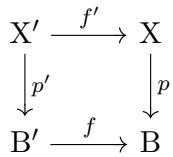
\includegraphics[keepaspectratio]{images/part001_2907af81.jpg}}

a Cartesian square.

\begin{enumerate}
\def\labelenumi{\alph{enumi})}
\item
  For every point \(b'\) of \(B'\) , the map \(f'\) induces a homeomorphism of the fiber \(X_{b'}'\) of \(p'\) onto the fiber \(X_{f(b')}\) of \(p\) .
\item
  If the map p is injective (resp. surjective, resp. bijective), then so is \(p'\) .
\end{enumerate}

Let \(b'\) be a point of B'. Set \(b = f(b')\) . For all \(x' \in X_{b'}'\) , we have \(p(f'(x')) = f(p'(x')) = f(b') = b\) , whence \(f'(x') \in X_b\) . This proves that one has \(X_{b'}' \subset \overline{f'}^{1}(X_b)\) . In Proposition 4, take \(B_0 = \{b\}\) , \(B_0' = \{b'\}\) and \(X_0 = X_b\) ; we then have \(X_0' = X_{b'}'\) , whence the assertion \(a\) ).

For the map p to be injective (resp. surjective, resp. bijective), it is necessary and sufficient that the cardinality of each of its fibers be at most (resp. at least, resp. equal to) 1. Assertion b) follows from this.

Example. --- Let \((X,p)\) be a B-space and A a subspace of B. The square

\[
\begin{array}{c} \overline {{p}} ^ {1} (\mathrm{A}) \xrightarrow {j} \mathrm{X} \\ \Biggl \downarrow p _ {\mathrm{A}} \\ \mathrm{A} \xrightarrow {i} \mathrm{B} \end{array}\tag{5}
\]

(where i and j are the canonical injections) is cartesian.

In particular, if A and A' are subspaces of the topological space B, the square

\begin{enumerate}
\def\labelenumi{(\arabic{enumi})}
\setcounter{enumi}{5}
\tightlist
\item
\end{enumerate}

\pandocbounded{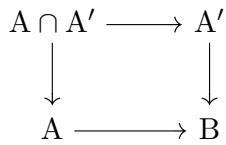
\includegraphics[keepaspectratio]{images/part001_a4278a10.jpg}}

(where the arrows are the canonical injections) is cartesian.

